\begin{frame}
\frametitle{Vertex Input}

\begin{itemize}
\item Quando creiamo un pipeline state object, specifichiamo il formato dei nostri vertici
\item In questo modo, la pipeline sa come interpretare i dati che abbiamo caricato
\end{itemize}

\begin{figure}[ht]
    \centering
    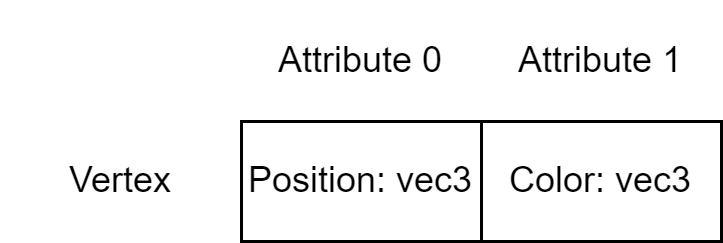
\includegraphics[scale=0.35]{images/SlidesVertices/VertexInputState.png}
\end{figure}

\end{frame}
